% Numeric source: paper/shared/evidence/raw/iclr_model_behavior/analysis_v1/results.json
\section{Disentangling Visual Dependence from the Output Interface}
\label{sec:mechanisms}

\paragraph{Where in the image does the change matter?}
We use rectangular-window crossovers to localize dependence on the changed
image. Let $W$ be the projected target box in the composed canvas. The
target-window condition replaces pixels in $W$ with their converted counterparts
while retaining the original context. The context-window condition makes the
opposite exchange. The two conditions are exact pixel interventions with the
same query, canvas, and target location. They separate sensitivity to the target
window from sensitivity to the surrounding visual evidence.

\begin{figure}[t]
\centering
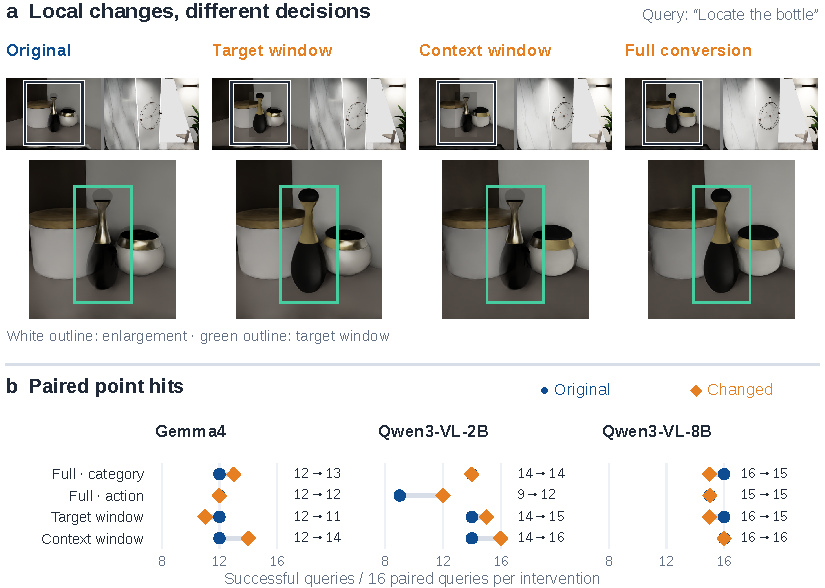
\includegraphics[width=\linewidth]{interventions.pdf}
\caption{Region crossovers and their grounding outcomes. Full canvases are
shown above matched enlargements. White outlines identify the enlargement;
green boxes mark the target window. The four columns show original,
target-window, context-window, and fully converted conditions. Annotations
are absent from model inputs. Paired counts use all 16 queries per condition.}
\label{fig:interventions}
\end{figure}

A converted scene changes both the target and the visual context in which it
appears. The crossover reveals whether changing one region reproduces the
response to full conversion, or instead pushes the prediction in another
direction.

Gemma4 provides a concrete example. Replacing the target window reduces success
from \GemmaTargetOrigPercent\% to \GemmaTargetConvPercent\%, whereas replacing the context increases it to \GemmaContextConvPercent\%.
The complete conversion yields \GemmaFullConvPercent\%. For Qwen3-VL-8B, the target-window
replacement introduces one miss and the context replacement retains all sixteen
hits. Qwen3-VL-2B instead reaches sixteen hits with converted context, compared
with fourteen in the original condition. These controlled outcomes show that
the location of the appearance change matters: target-window and contextual
changes can affect a model in different directions.

\paragraph{How is a location expressed?}
Output syntax and coordinate scale create a second mechanism for score changes.
Figure~\ref{fig:protocol} holds each set of raster inputs fixed across the
readout variants. Several configurations respond differently to pixel and
normalized requests. Molmo, for example, produces responses on a 0--100 scale in
some JSON/pixel prompts, while its two-line normalized prompts produce
0--1000-style points. Qwen3-VL-8B commonly retains a normalized-style output
even when asked for pixels. The raw responses reveal these scale mismatches before target-box scoring.

\begin{figure}[t]
\centering
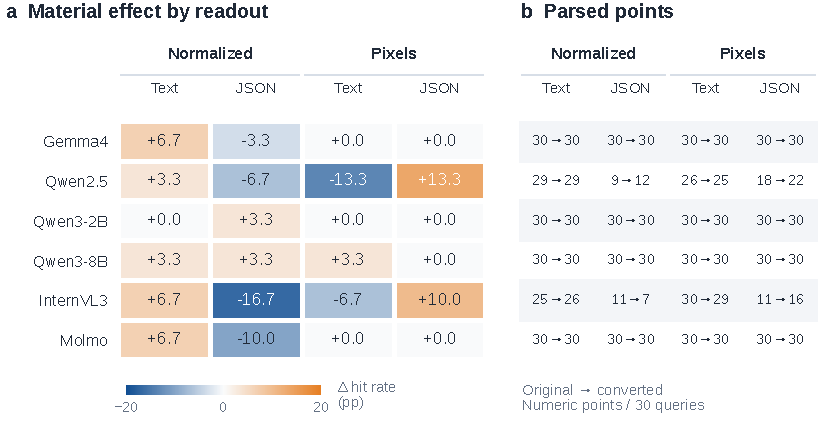
\includegraphics[width=\linewidth]{protocol.pdf}
\caption{Readout-dependent paired score changes in the 30-pair raster archive.
Each cell uses the requested coordinate frame and all 30 queries in each
condition. The heatmap reports percentage-point differences and the accompanying coverage
summary counts parsed numeric outputs. Full counts are in
Table~\ref{tab:protocol-full}.}
\label{fig:protocol}
\end{figure}

The response format therefore changes the meaning of a measured material
effect. A parser may discard a response, a coordinate mismatch may displace a
correctly identified location, or a valid point may genuinely move on the image.
Our analysis distinguishes these cases using raw text, explicit coordinate
transforms, and pixel distances. A miss caused by a scale mismatch therefore has a different explanation from
a point that moves off the object under a fixed readout.

\paragraph{Decoding variability.}
Three stochastic runs per image provide another view of spatial readout.
On the recorded raster inputs, Qwen3-VL-8B has a mean pairwise seed distance of
7.66 pixels, compared with 24.34 for Qwen3-VL-2B and 27.07 for Gemma4.
The corresponding hit-status variability is 0\%, 16.7\%, and 10.0\%.
Table~\ref{tab:sampling} gives the complete-query counts. These differences
motivate fixed decoding when comparing the two image conditions.
